% https://github.com/martinhelso/MathDept


\documentclass[UKenglish]{beamer}


\usetheme[NoLogo]{MathDept}


\usepackage[utf8]{inputenx} % For æ, ø, å
\usepackage{babel}          % Automatic translations
\usepackage{csquotes}       % Quotation marks
\usepackage{microtype}      % Improved typography
\usepackage{amssymb}        % Mathematical symbols
\usepackage{mathtools}      % Mathematical symbols
\usepackage{comment}        % Comment out multiple lines
\usepackage[absolute, overlay]{textpos} % Arbitrary placement
\setlength{\TPHorizModule}{\paperwidth} % Textpos units
\setlength{\TPVertModule}{\paperheight} % Textpos units
\usepackage{tikz}
\usetikzlibrary{snakes}
\usetikzlibrary{calc}
\usetikzlibrary{intersections}
\usetikzlibrary{decorations.markings}
\usetikzlibrary{decorations.pathreplacing,calligraphy}

\usetikzlibrary{overlay-beamer-styles}  % Overlay effects for TikZ

%Added by me 
\newcommand{\E}{\mathbb{E}}  % expectation
\newcommand{\F}{\mathcal{F}} % Filtration 

\newcommand{\R}{\mathbb{R}} % Real numbers


\author{Andreas Slåttelid}
\title{Advancements in Risk-Free Reference Rates and ESG-linked interest rate swaps}


\begin{document}


%\section{Overview}


% Use
%
%     \begin{frame}[allowframebreaks]{Title}
%
% if the TOC does not fit one frame.
\begin{frame}{Table of contents}
    \tableofcontents[currentsection]
\end{frame}


\section{Interest rate theory}
\subsection{Framework}

\begin{frame}{Framework}
\begin{itemize}
    \item $(\Omega, \F, P)$ probability space.  
    \item $\mathbb{F} = \{\F_{t}, t \in [0,T]\}$, right-continous and augmented, $T$ a fixed time horizon. 
    \item $W = \{W(t), t\in [0,T]\}$ a one-dimensional Brownian Motion. 
    \item $\mathcal{E} = \{\mathcal{E}_{t}(\gamma \bullet W), t \in [0,T]\}$ where: 
    \begin{align*}
     \mathcal{E}_{t}(\gamma \bullet W) := \exp\left(
     \int_{0}^{t}\gamma(s)dW(s) -\frac{1}{2}\int_{0}^{t}\gamma^{2}(s)ds
     \right)   
    \end{align*}
    \item We assume $ \E[\mathcal{E}_{t}(\gamma \bullet W)] = 1, \; \forall\;t\in [0,T]$ as well as the Novikov condition 
    \begin{align*}
     \E\left[
     \exp\left(
     \frac{1}{2}\int_{0}^{T}|\gamma(s)|^{2}ds
     \right)
     \right] < \infty   
    \end{align*}
\end{itemize}
\end{frame}


\begin{frame}{Framework}
\begin{itemize}
    \item This means that: 
    \begin{align*}
    \frac{dQ}{dP}\bigg{|}_{\F_{T}} := \mathcal{E}_{T}(\gamma \bullet W)   
    \end{align*}
    is well-defined, giving rise to a $Q$-Brownian Motion $W^{Q} = \{W^{Q}(t), t\in [0,T]\} $ defined on $(\Omega, \F, Q)$
\end{itemize} 
\end{frame}

\begin{frame}{Financial market}
\begin{itemize}
    \item $r = \{r(t), t\in [0,T]\}$ short-rate process such that $\int_{0}^{t}r(s)ds$ is well-defined, with $Q$-dynamics given by: 
    \begin{align*}
    dr(t) &= b(t,r(t))dt + \sigma(t,r(t))dW^{Q}(t)  \\
    r(0) &= r_{0} \in \R
    \end{align*}
    $b(t,x)$ and $\sigma(t,x)$ are assumed to be so 
    that the above SDE possess a unique and strong solution. 
    \item $B = \{B(t), t\in [0,T]\}$ the money market account, defined as: 
    \begin{align*}
        B(t) &= \exp\left(
        \int_{0}^{t}r(s)ds
        \right)
    \end{align*}
    \item $P(s,t)$ market value at time $s$ for a zero-coupon bond (ZCB) maturing at time $t,\; 0\leq s\leq t \leq T$. Guarantees its holder one unit of account at maturity. 
\end{itemize}
\end{frame}

\begin{frame}{Term Structure}
    \begin{itemize}
        \item A collection $\{P(s,t), 0\leq s \leq t \leq T\}$,  is called a term structure.
        \item Relationship between the short-rate and the ZCB:
        \begin{align*}
        P(t,T) &= \E_{Q}\left[
        \exp\left(
        -\int_{t}^{T}r(s)ds
        \right)\bigg{|}\F_{t}
        \right]    
        \end{align*}
    \item Assume that there exists a smooth function: 
    \begin{align*}
        g:\{(s,t)\in [0,T]\times [0,T]: s\leq t\}\times \R \to \R
    \end{align*}
    such that $P(s,t) = g(s,t,r(s))$. If: 
    \begin{align*}
    g(t,s,r(s)) &= \exp\left(
    -A(s,t)-B(s,t)r(s)
    \right)    
    \end{align*}
    we say that we have an affine term structure (ATS). ($A,B$ smooth $C^{1}$-functions).  
    \end{itemize}
\end{frame}

\begin{frame}{Interest rate swap}

An Interest Rate Swap (IRS) is a financial agreement between parties to exchange interest payments on a specific nominal $N$. The idea is to exchange floating and fixed rates.

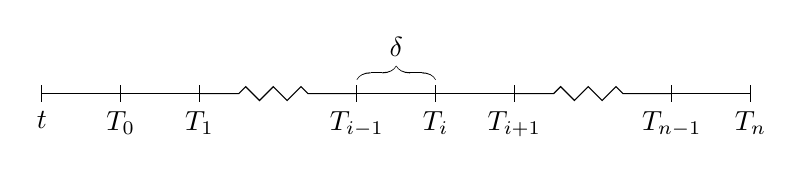
\begin{tikzpicture}[snake=zigzag, line before snake = 5mm, line after snake = 5mm]
    % draw horizontal line   
    \draw (0,0) -- (2,0);
    \draw[snake] (2,0) -- (4,0);
    \draw (4,0) -- (6,0);
    \draw[snake] (6,0) -- (8,0);
    \draw (8,0) -- (9,0);
    % Calligraphic brace
    \draw [
    decorate, 
    decoration = {calligraphic brace,
                  raise=5pt,
                  amplitude=5pt,
                  aspect=0.50}] (4,0) --  (5,0)
                  node[pos=0.50, above =1 0pt,black]{$\delta$};

    % draw vertical lines
    \foreach \x in {0,1,2,4,5,6,8,9}
      \draw (\x cm,3pt) -- (\x cm,-3pt);

    % draw nodes
    \draw (0,0) node[below=3pt] {$ t $} node[above=3pt] {$   $};
    \draw (1,0) node[below=3pt] {$ T_{0} $} node[above=3pt] {$  $};
    \draw (2,0) node[below=3pt] {$ T_{1} $} node[above=3pt] {$  $};
    \draw (3,0) node[below=3pt] {$  $} node[above=3pt] {$  $};
    \draw (4,0) node[below=3pt] {$ T_{i-1} $} node[above=3pt] {$  $};
    \draw (5,0) node[below=3pt] {$ T_{i} $} node[above=3pt] {$   $};
    \draw (6,0) node[below=3pt] {$ T_{i+1} $} node[above=3pt] {$  $};
    \draw (8,0) node[below=3pt] {$ T_{n-1} $} node[above=3pt] {$  $};
    \draw (9,0) node[below=3pt] {$ T_{n} $} node[above=3pt] {$  $};
  \end{tikzpicture}

\begin{itemize}
    \item $N$ nominal value. 
    \item $0 < T_{0} < T_{1} < \dots < T_{n}$ sequence of future dates. 
    \item $\delta := T_{i} - T_{i-1}$ fixed leg between payments. 
    \item $\kappa$ fixed rate 
    \item $F(T_{i-1}, T_{i})$ floating rate over $[T_{i-1}, T_{i}]$. 
\end{itemize}

The floating rate will reset at $T_{0}, \dots, T_{n-1}$ and the fixed rate will be paid at $T_{1}, \dots, T_{n}$. 
 
\end{frame}

\subsection{Interest rate swap}

\begin{frame}{Interest rate swap}
Perspective from payer IRS, at each instance $T_{i} , i = 1, \dots n$: 
\begin{itemize}
    \item Pay $\kappa \delta N$ (-)
    \item Receive $F(T_{i-1}, T_{i})\delta N$ (+)
\end{itemize}

Time-$t$ value $t\leq T_{0}$ of total cashflow: 

\begin{align*}
\pi(t) &= N[P(t,T_{0})- P(t,T_{n})] - \kappa \delta N \sum_{i=1}^{n}P(t,T_{i})     
\end{align*}

Now, the fixed swap-rate $\kappa = R_{Swap}(t)$, should be chosen such that $\pi(t) = 0$, namely: 
\begin{align*}
\kappa &= \frac{
P(t,T_{0}) - P(t,T_{n})
}{
\delta \sum_{i=1}^{n}P(t,T_{i})
}    
\end{align*}

\end{frame}



\begin{comment}
\begin{frame}{Framework}
    \begin{theorem}[Fermat's little theorem]
        For a prime~\(p\) and \(a \in \mathbb{Z}\) it holds that \(a^p \equiv a \pmod{p}\).
    \end{theorem}
    
    \begin{proof}
        The invertible elements in a field form a group under multiplication.
        In particular, the elements
        \begin{equation*}
            1, 2, \ldots, p - 1 \in \mathbb{Z}_p
        \end{equation*}
        form a group under multiplication modulo~\(p\).
        This is a group of order \(p - 1\).
        For \(a \in \mathbb{Z}_p\) and \(a \neq 0\) we thus get \(a^{p-1} = 1 \in \mathbb{Z}_p\).
        The claim follows.
    \end{proof}

\end{frame}
\end{comment}



%\subsection{Example}


\begin{frame}{Mathematics}
    \begin{example}
        The function \(\phi \colon \mathbb{R} \to \mathbb{R}\) given by \(\phi(x) = 2x\) is continuous at the point \(x = \alpha\),
        because if \(\epsilon > 0\) and \(x \in \mathbb{R}\) is such that \(\lvert x - \alpha \rvert < \delta = \frac{\epsilon}{2}\),
        then
        \begin{equation*}
            \lvert \phi(x) - \phi(\alpha)\rvert = 2\lvert x - \alpha \rvert < 2\delta = \epsilon.
        \end{equation*}
    \end{example}
\end{frame}


\section{Highlighting}
\SectionPage


\begin{frame}{Highlighting}
    Some times it is useful to \alert{highlight} certain words in the text.
    
    \begin{alertblock}{Important message}
        If a lot of text should be \alert{highlighted}, it is a good idea to put it in a box.
    \end{alertblock}
    
    It is easy to match the \structure{colour theme}.
\end{frame}


\section{Lists}


\begin{frame}{Lists}
    \begin{itemize}
        \item
        Bullet lists are marked with a grey box.
    \end{itemize}
    
    \begin{enumerate}
        \item
        \label{enum:item}
        Numbered lists are marked with a white number inside a grey box.
    \end{enumerate}

    \begin{description}
        \item[Description]
        highlights important words with grey text.
    \end{description}

    Items in numbered lists like \enumref{enum:item} can be referenced with a grey box.

    \begin{example}
        \begin{itemize}
            \item
            Lists change colour after the environment.
        \end{itemize}
    \end{example}
\end{frame}


\section{Effects}
hei 

\section{References}


\begin{frame}[allowframebreaks]{References}
    \begin{thebibliography}{}

        % Article is the default.
        \setbeamertemplate{bibliography item}[book]

        \bibitem{Hartshorne1977}
        Hartshorne, R.
        \newblock \emph{Algebraic Geometry}.
        \newblock Springer-Verlag, 1977.

        \setbeamertemplate{bibliography item}[article]

        \bibitem{Helso2020}
        Helsø, M.
        \newblock \enquote{Rational quartic symmetroids}.
        \newblock \emph{Adv. Geom.}, 20(1):71--89, 2020.

        \setbeamertemplate{bibliography item}[online]

        \bibitem{HR2018}
        Helsø, M.\ and Ranestad, K.
        \newblock \emph{Rational quartic spectrahedra}, 2018.
        \newblock \url{https://arxiv.org/abs/1810.11235}

        \setbeamertemplate{bibliography item}[triangle]

        \bibitem{AM1969}
        Atiyah, M.\ and Macdonald, I.
        \newblock \emph{Introduction to commutative algebra}.
        \newblock Addison-Wesley Publishing Co., Reading, Mass.-London-Don
        Mills, Ont., 1969

        \setbeamertemplate{bibliography item}[text]

        \bibitem{Artin1966}
        Artin, M.
        \newblock \enquote{On isolated rational singularities of surfaces}.
        \newblock \emph{Amer. J. Math.}, 80(1):129--136, 1966.

    \end{thebibliography}
\end{frame}


\end{document}